
\documentclass[letterpaper, 10 pt, conference]{ieeeconf}  % Comment this line out if you need a4paper

%\documentclass[a4paper, 10pt, conference]{ieeeconf}      % Use this line for a4 paper

\IEEEoverridecommandlockouts                           

\overrideIEEEmargins                                      % Needed to meet printer requirements.

%In case you encounter the following error:
%Error 1010 The PDF file may be corrupt (unable to open PDF file) OR
%Error 1000 An error occurred while parsing a contents stream. Unable to analyze the PDF file.
%This is a known problem with pdfLaTeX conversion filter. The file cannot be opened with acrobat reader
%Please use one of the alternatives below to circumvent this error by uncommenting one or the other
%\pdfobjcompresslevel=0
%\pdfminorversion=4

% See the \addtolength command later in the file to balance the column lengths
% on the last page of the document

% The following packages can be found on http:\\www.ctan.org
\usepackage{graphics} % for pdf, bitmapped graphics files
\usepackage{epsfig} % for postscript graphics files
\usepackage{mathptmx} % assumes new font selection scheme installed
\usepackage{times} % assumes new font selection scheme installed
\usepackage{tabularx}
\usepackage{graphicx}
\usepackage{amsmath}
\usepackage{amsfonts}
\usepackage{amssymb}
\usepackage{url}
\usepackage{cite}
\usepackage{threeparttable}
\usepackage{multirow}

\PassOptionsToPackage{hyphens}{url}
\usepackage{hyperref}


\title{\LARGE \bf
Tracking Psychological Risk in Alzheimer’s Caregivers: A Comparison of Machine Learning and Large Language Models
}


\author{%
Junen Xiao$^{1*}$%
\thanks{$^{1}$Junen Xiao is with the Department of Electrical and Computer Engineering, Rice University, Houston, TX 77005, USA (\texttt{jx57@rice.edu}).}%
}


\begin{document}

\maketitle
\thispagestyle{empty}
\pagestyle{empty}


%%%%%%%%%%%%%%%%%%%%%%%%%%%%%%%%%%%%%%%%%%%%%%%%%%%%%%%%%%%%%%%%%%%%
\begin{abstract}
Spousal caregivers of individuals with Alzheimer's disease frequently experience a high caregiver burden and loneliness, leading to sustained psychological stress. Given the association between chronic caregiving stress and adverse health outcomes, early identification of psychological risk in caregivers is essential for prevention.

Current approaches for stress inference typically rely on data from wearable sensors, together with standardized psychological scales. To capture the multidimensional nature of mental health, state-of-the-art approaches adopt multimodal modeling to improve predictive performance.

In this study, we integrate wearable-derived features and interview-based text to classify caregivers psychological risk levels using the Perceived Stress Scale, Zarit Burden Interview, and UCLA Loneliness Scale. We compare performance of traditional machine learning models and large language models (Gemini 2.0, Llama 4, and GPT-4o) across different modality settings and prompting strategies. 
\end{abstract}


%%%%%%%%%%%%%%%%%%%%%%%%%%%%%%%%%%%%%%%%%%%%%%%%%%%%%%%%%%%%%%%%%%%%%%%%%%%%%%%%
\section{INTRODUCTION}
Caring for a spouse with Alzheimer's Disease and Alzheimer's Disease Related Dementias (AD/ADRD) constitutes a major source of emotional strain\cite{stress}. This chronic caregiving stress is linked to physiological stress responses, including increased pro-inflammatory activity and systemic inflammation, which can lead to adverse health outcomes\cite{caregivingstress,family}. These effects often develop gradually and may not be immediately apparent in daily life\cite{immediate}. Therefore, timely detection of rising psychological strain is essential. However, caregivers vary substantially in their resilience and vulnerability to stress\cite{resilience}. This emphasizes the need for personalized, timely stress detection to identify individuals at elevated risk and enable targeted support.

Validated self-report instruments such as the Perceived Stress Scale (PSS)\cite{pss}, Zarit Burden Interview (ZBI)\cite{ZBI}, and UCLA Loneliness Scale (UCLALS)\cite{ucla} are commonly used to assess caregiver psychological risk in caregiving studies. However, these surveys are typically administered infrequently due to participant burden\cite{surveyburden}, which limits the ability to capture important fluctuations in psychological status over time. 

Passive sensing data from wearable devices, which capture continuous behavioral and physiological signals, provide rich insights into stress-related processes \cite{smets2018large}. However, wearable-derived data alone may not adequately capture the subjective psychological experiences central to caregiving. This has motivated recent studies to leverage textual data to estimate standard self-report psychological scales \cite{textwellbeing}.

More recently, several studies have explored the use of large language models (LLMs) for mental health state prediction \cite{xu2024mental,yang2023towards,lamichhane2023evaluation}, with prompt engineering emerging as a commonly adopted approach. For example, Xu et al.~\cite{xu2024mental} and Yang et al.~\cite{yang2023towards} leveraged human-annotated mental health text from social media platforms (e.g., Reddit) to evaluate the effectiveness of different prompting strategies. Their work examined a range of approaches, including zero-shot, few-shot, and emotion-aware prompting, and demonstrated that prompt design can significantly influence LLM performance.


Based on the above motivations, our contributions can be summarized as follows:
\begin{itemize}
\item We systematically compare traditional machine learning models and LLMs for classifying AD/ADRD caregivers into high vs.\ low groups across three psychological scales (PSS, ZBI, and UCLALS).

\item We evaluate traditional machine learning approaches under multiple modality settings, including wearable-only, interview-only, and multimodal configurations.

\item We design six prompting strategies for LLMs (Gemini 2.0, Llama 4, and GPT-4o) and evaluate their performance across different modality settings.

\end{itemize}


\section{Method}
\subsection{Dataset}
This study enrolled 32 caregivers (28 female and 4 male) of patients with Alzheimer’s disease. The inclusion criteria for AD/ADRD spousal caregivers are as follows: (1) self-identified as the primary caregiver of a spouse with dementia; (2) providing at least 4 hours of daily care for a minimum of the past 3 months; (3) the caregiver and the AD/ADRD patient have been married or in a self-defined long-term committed relationship for at least 3 years.

Participants wore Fitbit devices during a 7-day study block, which continuously recorded minute-level heart rate, sleep status, and step count data. At the end of the study, participants completed a 30-minute interview consisting of 28 questions. These questions covered categories such as caregiving background, caregiving experiences, and stress levels. Participants also completed the standardized surveys (PSS-10\cite{pss}, UCLALS Version 3\cite{ucla}, and ZBI-13\cite{ZBI}), which served as ground-truth labels in this study. 

\subsection{Interview Data Processing}
Transcripts were generated offline from the interview audio using OpenAI Whisper\cite{radford2023robust}. Coders reviewed the text, segmented the interviews into meaningful units, anonymized identifiable information, and cleaned the transcripts by removing filler words and other non-informative content.

\subsection{Wearable Feature Extraction}
\begin{figure}[!t]
    \centering
    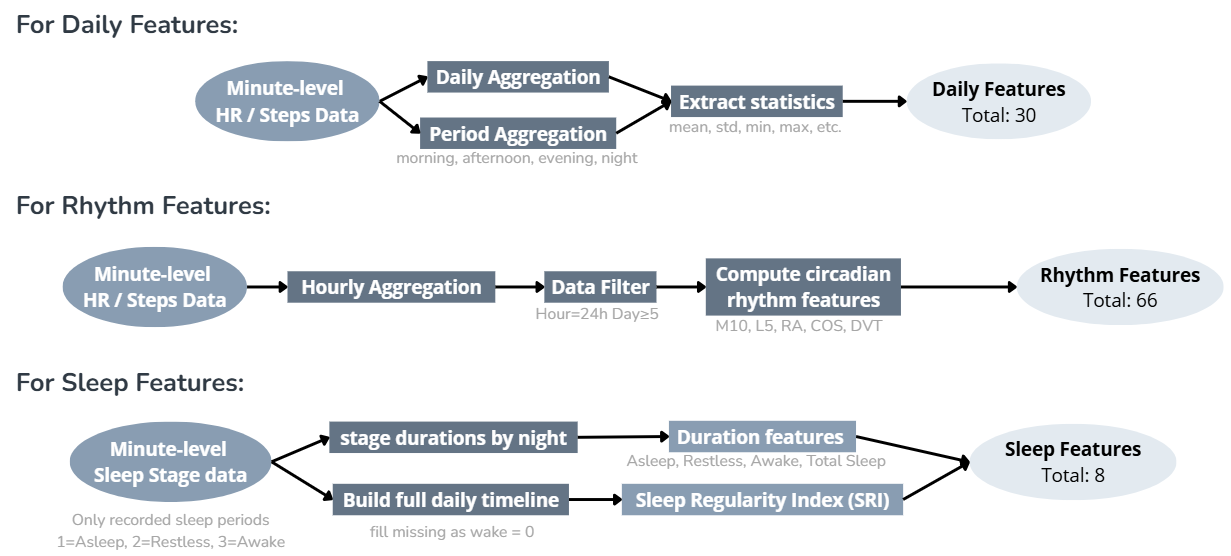
\includegraphics[width=\linewidth]{FeatureExtraction.png}
    \caption{Overview of the feature selection workflow.}
    \label{fig:feature_workflow}
\end{figure}
We extracted sleep, daily, and rhythm features from the Fitbit data of each participant. Fig.~\ref{fig:feature_workflow} shows the feature extraction process. Sleep features mainly consist of the duration in different stages of sleep, including asleep, restless, and awake states. The Sleep Regularity Index (SRI)~\cite{sri} was also calculated based on the whole-day sleep states at minute-level resolution. The higher SRI indicates greater regularity in sleep patterns.

Daily features were derived from minute-level heart rate and step data, stress-related physiological responses, and daily activity patterns. Heart rate features included summary statistics and the proportion of minutes with elevated heart rate (HR$>$100 bpm). This is because elevated heart rate may indicate periods of increased physiological stress or activation\cite{schneider2021life}. Activity features included step statistics, active and sedentary time proportions, and step entropy. Features were computed separately for different times of day (morning, afternoon, evening, and night).

Rhythm features were extracted from hourly aggregated heart rate and step data, which reflect individuals’ circadian regularity and the stability of their daily physiological and behavioral patterns\cite{smagula2022association}.  The features have been shown to be associated with health and stress outcomes\cite{relationshipZBI,smagula2022association,heartrate}. To ensure reliable estimation, participants with at least five complete days of 24-hour data were included. Rhythm features were then derived using both nonparametric metrics and parametric cosinor analysis. Additional statistics describing deviations from the participant-specific 24-hour activity template were computed to capture rhythm stability and variability. 

In total, 104 features were extracted, including  8 sleep features, 30 daily features and 66 rhythm features. 

\subsection{Machine Learning Models}
We utilized traditional machine learning models including Support Vector Machine (SVM)\cite{cortes1995support}, XGBoost (XGB)\cite{xgboost}, Random Forest (RF)\cite{rf}, and K-Nearest Neighbors (KNN)\cite{knn}  due to their robustness and suitability for small-sample settings. These models are trained to classify participants into different risk groups under different modality configurations for PSS, ZBI and UCLALS respectively. 

Due to the limited sample size (n = 32), Leave-One-Out Cross-Validation (LOOCV)\cite{loocv} was employed, where one participant was held out as the test sample and the remaining participants were used for training. After 32 folds, each participant was used exactly once as the test sample. The predictions from all folds were then aggregated to compute the overall evaluation metrics.

\begin{figure}[!t]
    \centering
    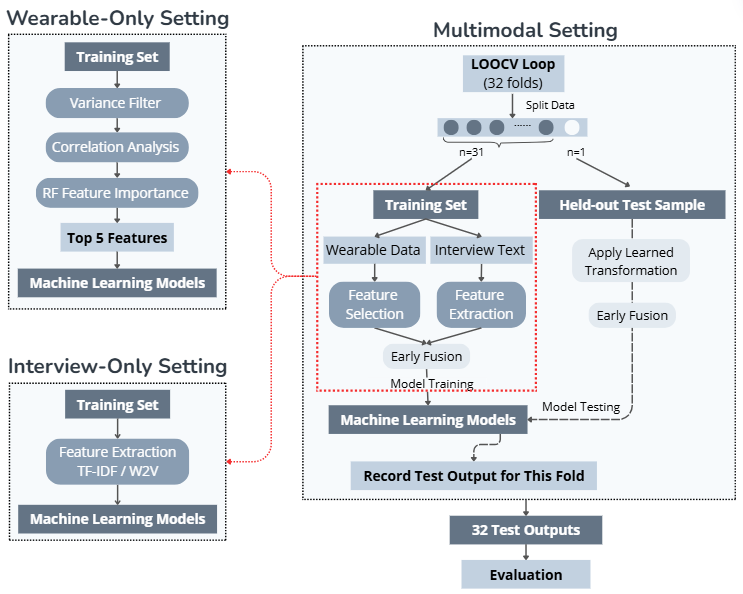
\includegraphics[width=\linewidth]{Feature_Selection.png}
    \caption{LOOCV-based machine learning models training pipeline.}
    \label{fig:feature_selection}
\end{figure}

Wearable feature selection was performed within each training fold using only the training data, including low-variance filtering, correlation analysis, and Random Forest-based importance ranking, with the top five features retained. For interview text, TF-IDF \cite{tf-idf} or Word2Vec (W2V) \cite{word2vec} was applied within each training fold, and the learned transformations were used to process the corresponding test samples without refitting. Multimodal features were constructed by concatenating text and wearable features within each fold. Fig.~\ref{fig:feature_selection} illustrates the LOOCV-based pipeline for model training and evaluation.

\subsection{Prompt Engineering Strategies}
An LLM-based approach was also adopted for identification of different risk levels among participants. In this framework, interview transcripts and wearable features were integrated at the prompt level. Specifically, the interview text was provided directly as natural language input, while wearable features were converted into textual descriptions with feature names, explanations, and numeric values. These multimodal inputs were then combined within a single prompt to guide the model to classify the participants.

Given that LLM predictions can be sensitive to the instructed perspective \cite{patient}, we designed prompt engineering strategies based on two distinct perspectives: a caregiver-centered perspective and a clinical psychometrician perspective. Under the caregiver-centered perspective, the LLM is prompted to interpret the input (interview text or wearable-derived features) by imagining itself as the caregiver and reflecting on their subjective experience. In contrast, under the expert perspective, the LLM is instructed to assess risk as a clinical psychometrician based on the provided data.

We also designed two task-framing strategies: direct classification and score prediction. In the direct classification setting, predefined cutoff values for each psychological scale were provided, and the LLMs were instructed to directly output a binary risk label. In the score prediction setting, the LLMs first predicted scale scores, which were then converted into binary labels based on the corresponding cutoffs. 

By varying access to each questionnaire item under the clinical psychometrician perspective, we further explored informed and uninformed strategies. In the informed setting, the LLM was provided with the full set of questionnaire items, whereas in the uninformed setting, only the scale range and cutoff information were available. Fig.~\ref{fig:prompt_engineering} provides an overview of the prompt engineering strategies. These strategies were used to conduct zero-shot inference with three models: Gemini~2.0, GPT-4o, and Llama~4.

\begin{figure}[t]
    \centering
    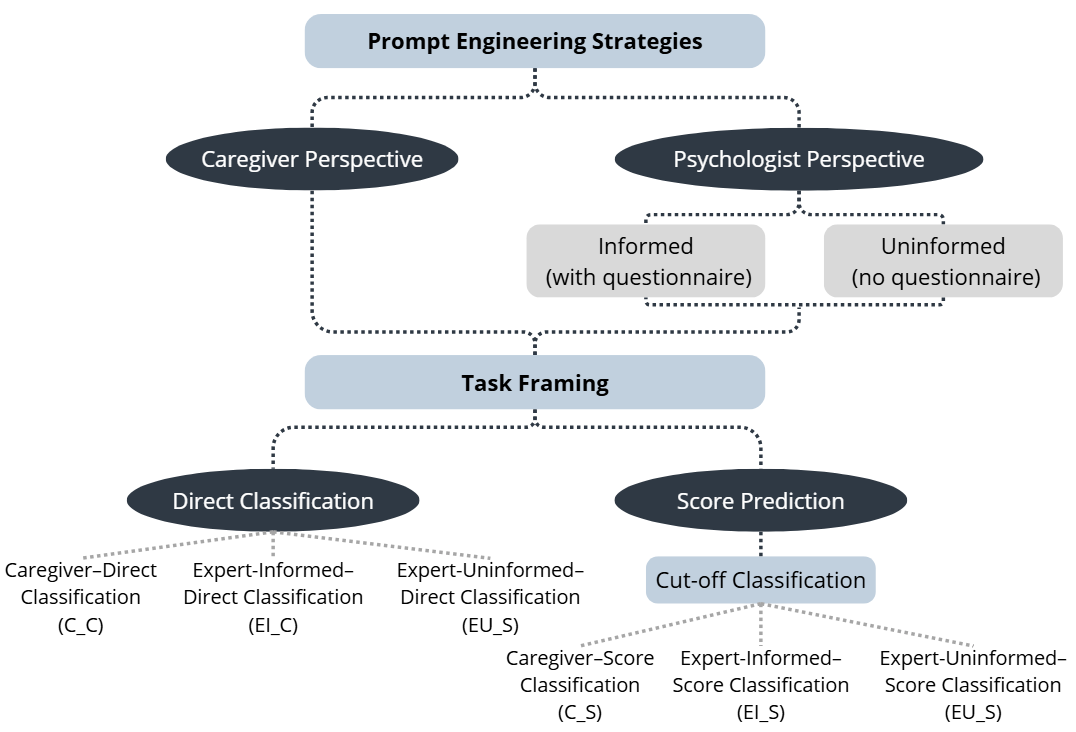
\includegraphics[width=\linewidth]{Prompt_Engineering.png}
    \caption{Overview of the prompt engineering strategies.}
    \label{fig:prompt_engineering}
\end{figure}

\subsection{Evaluation}
The performance of traditional machine learning models and LLM-based approaches was evaluated using accuracy, recall, F1-score, and precision. 

For LLM-based approaches, the zero-shot predictions were directly compared with ground truth labels to compute evaluation metrics. Due to the differences in task formulation across prompting strategies, outputs from score prediction tasks were first converted into binary labels based on clinical cutoffs before evaluation. To account for variability in LLM outputs, results are reported as the mean and standard deviation over five runs. 

\section{RESULTS}
\subsection{Participant Characteristics }
Among the 32 participants, 28 were female, and 4 were male, with ages ranging from 50 to 89 years (mean = 71, SD = 7.04). Most participants identified as White (n = 27), followed by African American (n = 4) and Other (n = 1). The majority were retired (n = 24), with fewer participants employed full-time (n = 4) or part-time (n = 2), and only few participants were unemployed (n = 1) or reported being disabled (n = 1). Most participants had children or stepchildren (n = 24), while a smaller proportion did not (n = 8).

In addition, we examined the basic statistics of the three assessment scales. The PSS scores ranged from 6 to 30, with a mean of 16.78 (SD = 6.28), suggesting moderate variability in perceived stress levels among participants. The ZBI scores ranged from 8 to 37, with a mean of 21.72 (SD = 7.78), while the UCLALS scores had a mean of 41.38 (SD = 9.83). 

This indicates that a substantial proportion of caregivers experienced relatively high levels of burden and loneliness. We categorized participants into two groups using established cut-off criteria for the 3 scales, respectively. The binary classification criteria and label distribution for the psychological scales are summarized in Table~\ref{tab:label_distribution}.

\begin{table}[t]
\centering
\caption{Binary classification rules and label distribution for psychological scales.}
\label{tab:label_distribution}
\begin{tabular}{lccc}
\hline
\textbf{Scale} & \textbf{Binary Rule} & \textbf{Low Risk (n,\%)} & \textbf{High Risk (n,\%)} \\
\hline
PSS\cite{pss} & $\geq 14 \rightarrow 1$ & 10 (31.25\%) & 22 (68.75\%) \\
UCLALS\cite{ucla} & $\geq 35 \rightarrow 1$ & 8 (25.00\%) & 24 (75.00\%) \\
ZBI\cite{ZBI} & $\geq 21 \rightarrow 1$ & 12 (37.50\%) & 20 (62.50\%) \\
\hline
\end{tabular}
\end{table}

\subsection{Impact of Modality on Prediction Performance}
To better understand the impact of different input modalities (Wearable Only, Interview Only, and Multimodal), we selected the best-performing traditional machine learning method,  and conducted comparisons across modalities. For LLM-based approaches, we performed one-way ANOVA on Accuracy, F1-score, and Precision over 5 runs, as they reflect overall performance and prediction quality. Recall was not included due to its minimal variation across modalities. We then conducted post-hoc Tukey HSD tests to examine pairwise differences.

Table~\ref{tab:ml_results} shows the performance of traditional machine learning methods under different modality configurations. Overall, the Wearable Only setting achieves the best performance, as it consistently yields strong results across all three scales. For UCLALS, the multimodal method outperforms other modalities, with the highest accuracy of 0.81. In contrast, for PSS, the Interview Only and Wearable Only settings show comparable performance. For ZBI, both the Interview Only and Multimodal settings perform much worse compared to Wearable Only.

Fig.~\ref{fig:anova_llm} compares LLM performance across modality settings (multimodal, wearable-only, and interview-only), where all configurations are evaluated using the same LLM (Gemini~2.0) and a consistent prompt engineering strategy within each scale. Overall, LLMs achieved the best performance under the Interview Only setting, with accuracy reaching 0.81 on ZBI, whereas performance degraded substantially under the Wearable Only setting, with the lowest accuracy observed on UCLALS (0.28).

We also report statistical significance in Fig.~\ref{fig:anova_llm}, where modality has a significant effect on Accuracy, F1-score, and Precision for both PSS and ZBI. while for UCLALS, significance is observed only in Precision. The Tukey HSD results further indicate that, for UCLALS, the significant difference in Precision is primarily driven by the comparison between the Wearable Only and Multimodal settings. 

\begin{table}
\caption{Performance of Traditional Machine Learning Methods Across Different Modalities}
\label{tab:ml_results}
\centering
\begin{threeparttable}
\begin{tabular}{llccc}
\hline
\textbf{Scale} & \textbf{Method} & \textbf{Accuracy} & \textbf{F1} & \textbf{Precision} \\
\hline

\multirow{3}{*}{PSS}
& Multimodal (KNN) & 0.62 & 0.76 & 0.68 \\
& Wearable (KNN) & 0.78 & 0.85 & 0.80 \\
& Interview (KNN) & 0.75 & 0.85 & 0.73 \\
\hline

\multirow{3}{*}{ZBI}
& Multimodal (XGBoost) & 0.53 & 0.67 & 0.60 \\
& Wearable (XGBoost) & 0.72 & 0.79 & 0.74 \\
& Interview(XGBoost) & 0.59 & 0.72 & 0.63 \\
\hline

\multirow{3}{*}{UCLALS}
& Multimodal (SVM) & 0.81 & 0.88 & 0.85 \\
& Wearable (SVM) & 0.78 & 0.84 & 0.91 \\
& Interview (SVM) & 0.66 & 0.79 & 0.72 \\
\hline

\end{tabular}
\end{threeparttable}
\end{table}

\begin{figure}[t]
\centering
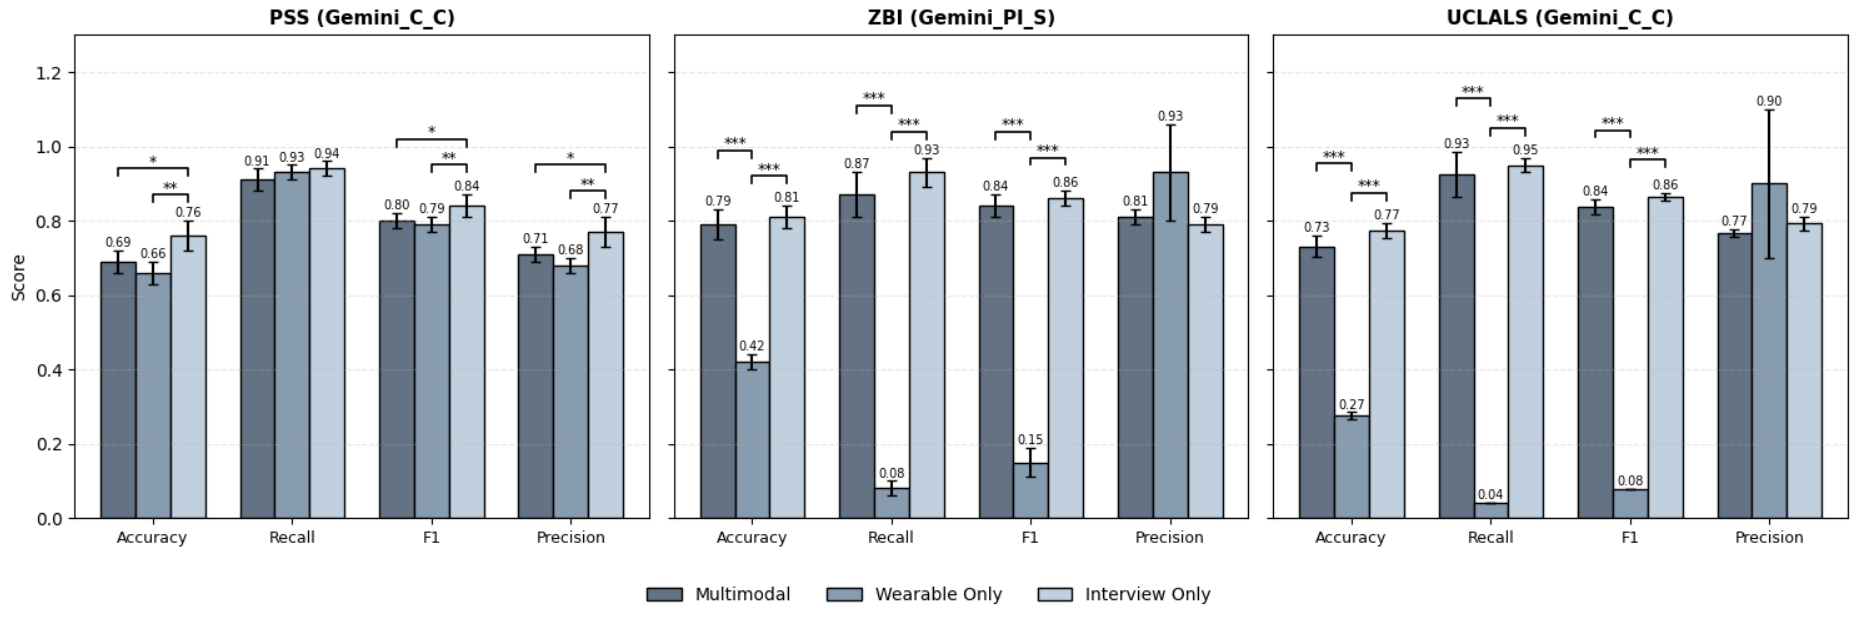
\includegraphics[width=\linewidth]{ANOVA_LLM.png}
\caption{LLM performance comparison across modality settings (multimodal, wearable-only, interview-only), with statistical significance indicated (* $p<0.05$, ** $p<0.01$, *** $p<0.001$).}
\label{fig:anova_llm}
\end{figure}

\subsection{Performance of Traditional Machine Learning Models and Contributing Features}
\begin{figure}[t]
\centering
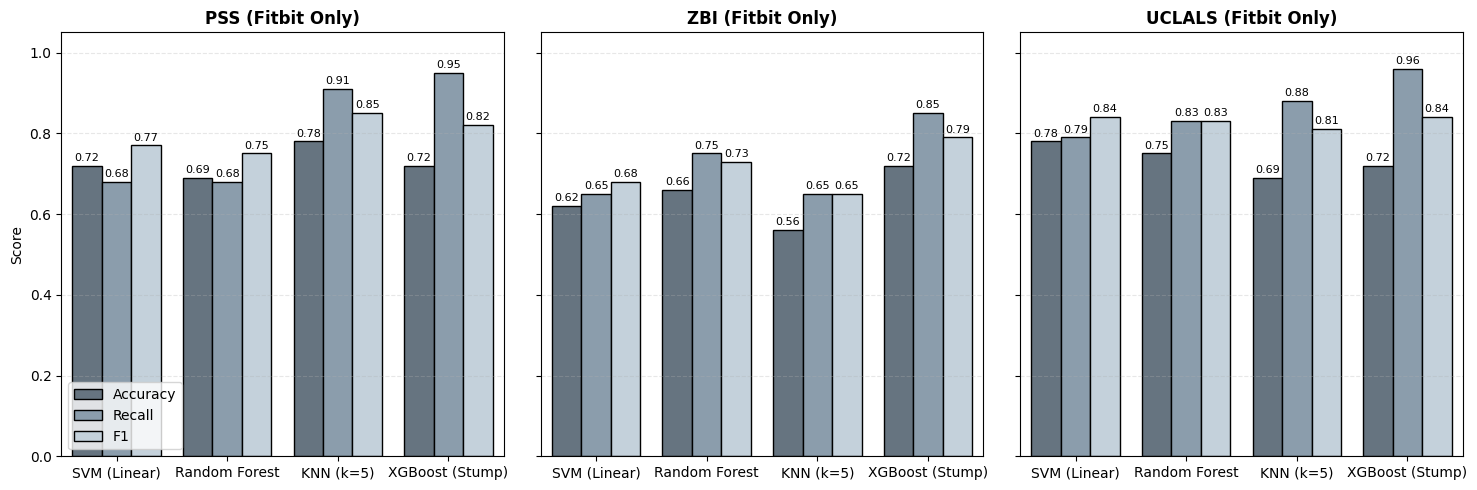
\includegraphics[width=\linewidth]{ML.png}
\caption{Comparison of machine learning models across PSS, ZBI, and UCLALS under the wearable-only setting.}
\label{fig:ml_wearable}
\end{figure}
The above analysis shows that traditional machine learning models achieved the best performance under the Wearable-only setting. Fig.~\ref{fig:ml_wearable} presents the performance of different models across multiple scales using Wearable features. For the PSS task, KNN achieved the best performance, reaching an accuracy of 0.78 and a recall of 0.85. For the ZBI task, XGBoost performed best with an accuracy of 0.72. For the UCLALS task, SVM achieved the highest accuracy of 0.78.

To further understand which features contributed most to model predictions, we conducted a SHAP-based feature importance analysis using XGBoost under the wearable-only setting for all three scales. As shown in Fig.~\ref{fig:fitbit_shap}, activity levels, heart rate variability, circadian rhythm characteristics, and sleep-related measures all played key roles in the model predictions.

\begin{figure}[t]
\centering
\includegraphics[width=\linewidth]{SHAP.png}
\caption{SHAP-based feature importance for the wearable-only (Fitbit) setting across PSS, ZBI, and UCLALS.}
\label{fig:fitbit_shap}
\end{figure}


The TF-IDF feature importance under a linear SVM model for each task is shown in Fig.~\ref{fig:tfidf_features}. PSS-related features were mainly associated with caregiving contexts and descriptions of daily routines, while ZBI features reflected caregiving challenges and external stressors. In contrast, UCLALS features were more related to communication and emotional perception.  

\begin{figure}[t]
    \centering
    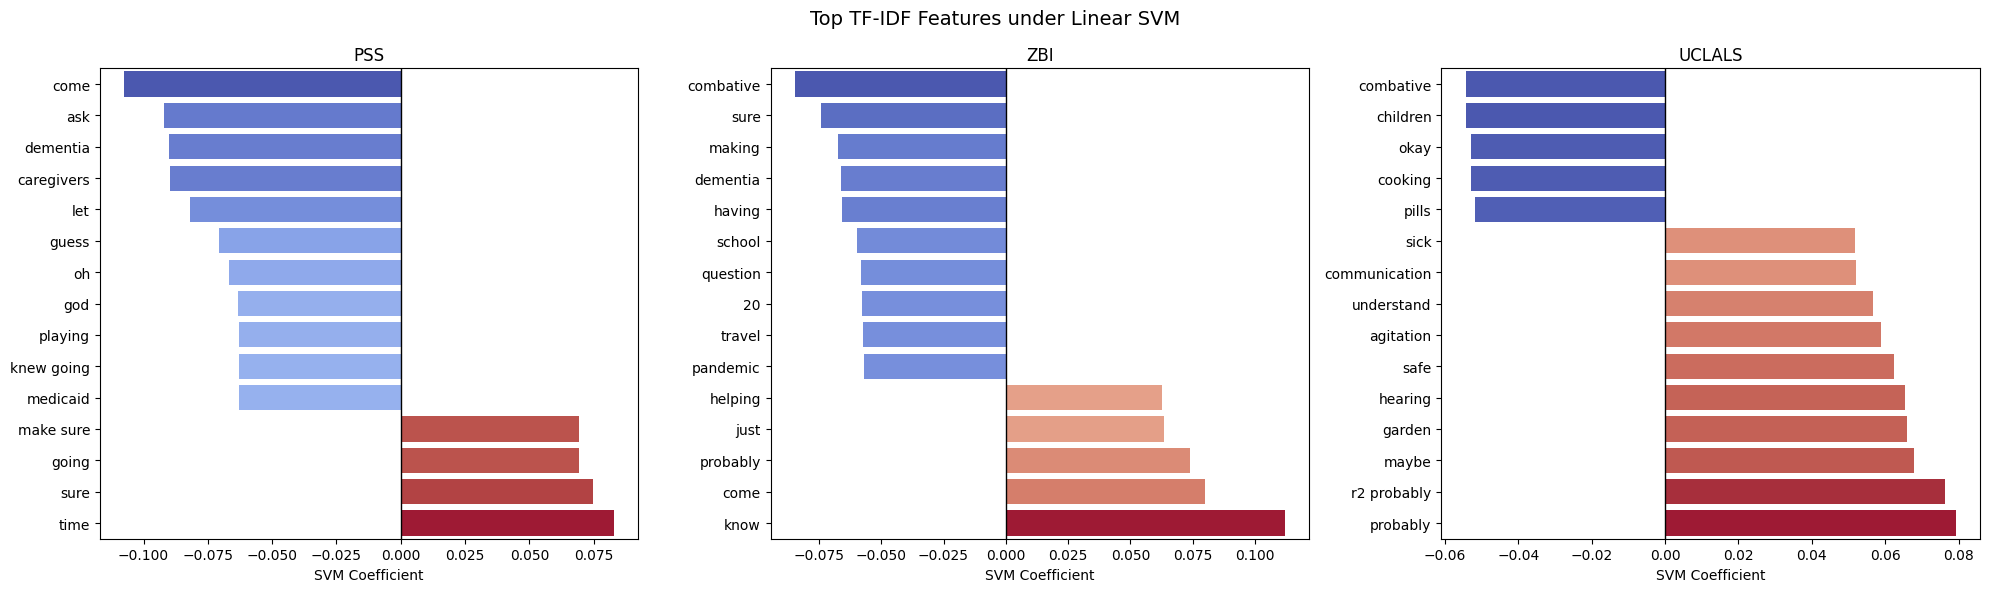
\includegraphics[width=\linewidth]{TF-IDF.png}
    \caption{Top TF-IDF features for PSS, ZBI, and UCLALS under the interview-only setting.}
    \label{fig:tfidf_features}
\end{figure}

\subsection{Performance of Large Language Models(LLMs)}
\subsubsection{Effect of Prompt Engineering Strategies}
\begin{table}
\caption{Performance comparison of different prompt engineering strategies for ZBI under multimodal setting.}
\label{tab:zbi_prompt}
\centering
\begin{threeparttable}
\begin{tabular}{lccc}
\hline
\textbf{Method} & \textbf{Accuracy} & \textbf{F1} & \textbf{Precision} \\
\hline
Gemini\_C\_S  & 0.76 $\pm$ 0.04 & 0.84 $\pm$ 0.03 & 0.73 $\pm$ 0.03 \\
Gemini\_C\_C  & \textbf{0.81 $\pm$ 0.02} & \textbf{0.87 $\pm$ 0.01} & 0.76 $\pm$ 0.02 \\
Gemini\_PI\_S & 0.79 $\pm$ 0.04 & 0.84 $\pm$ 0.03 & \textbf{0.81 $\pm$ 0.02} \\
Gemini\_PI\_C & 0.79 $\pm$ 0.04 & 0.85 $\pm$ 0.03 & 0.76 $\pm$ 0.02 \\
Gemini\_PU\_S & 0.77 $\pm$ 0.03 & 0.83 $\pm$ 0.03 & 0.78 $\pm$ 0.01 \\
Gemini\_PU\_C & 0.69 $\pm$ 0.02 & 0.82 $\pm$ 0.01 & 0.75 $\pm$ 0.02 \\
\hline
\end{tabular}
\end{threeparttable}
\end{table}
Due to the difficulty of identifying a consistently superior prompt engineering strategy across all settings, we analyze the performance of the ZBI (multimodal) task under six different prompting strategies, with results shown in Table~\ref{tab:zbi_prompt}.

We further conduct one-way ANOVA and post-hoc Tukey HSD tests for ZBI under the multimodal setting. The results indicate that the psychometrician-informed score-based strategy (PI\_S) is the most stable approach, achieving consistently strong performance across accuracy, precision, and specificity. In contrast, the psychometrician-uninformed classification strategy (PU\_C) performs the worst overall, with significantly lower accuracy and specificity.

\subsubsection{Comparison on Different LLMs}
\begin{figure}[t]
\centering
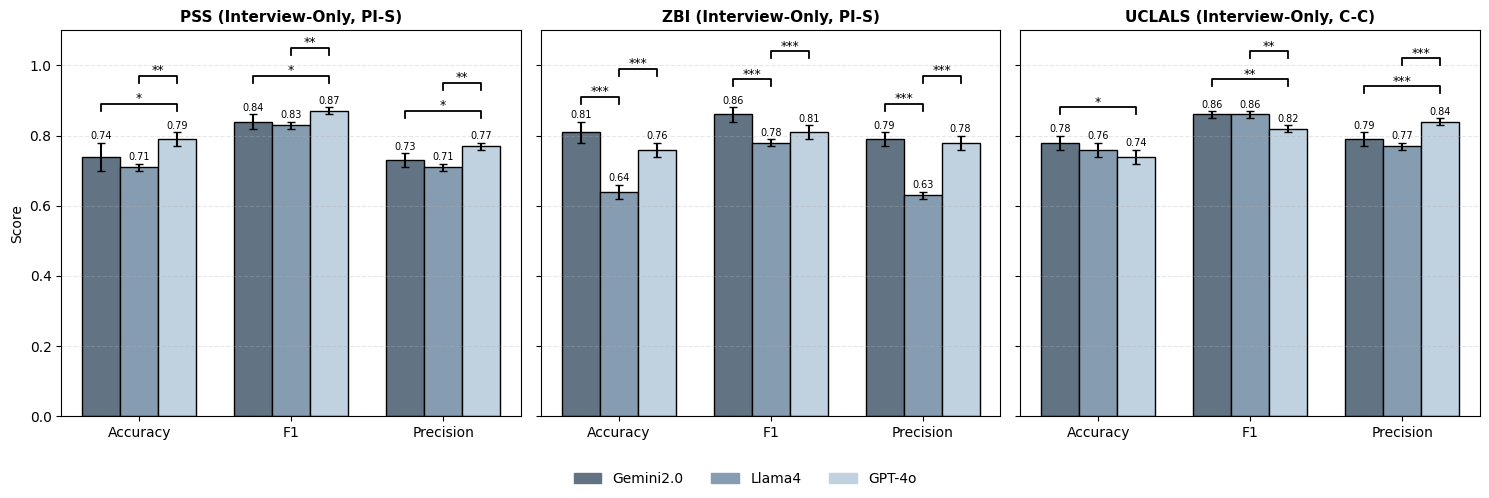
\includegraphics[width=\linewidth]{LLM.png}
\caption{Comparison of performance of different LLMs across PSS, ZBI, and UCLALS under the Interview Only setting, with statistical significance indicated (* $p<0.05$, ** $p<0.01$, *** $p<0.001$).}
\label{fig:llm_comparison}
\end{figure}
To conduct a fair performance comparison across different LLMs,  we evaluate Gemini~2.0, GPT-4o, and Llama~4 under consistent experimental conditions, using  Interview Only and consistent prompt strategies for each scale. For PSS and ZBI, we use the psychometrician-informed score-based strategy (PI\_S), while for UCLALS, we adopt the caregiver-based direct classification strategy (C\_C). Figure~\ref{fig:llm_comparison} presents the results, where all metrics are reported as mean values over five runs.

Overall, Llama~4 shows slightly lower performance than the other two models on both PSS and ZBI, while achieving comparable better performance on UCLALS. This may be attributed to the class imbalance in the UCLALS dataset. For PSS, GPT-4o achieves the best performance, with an accuracy of 0.79 and an F1 score of 0.87. In contrast, Gemini~2.0 performs best on ZBI and UCLALS, with the highest accuracy of 0.81 on ZBI. 

\section{Discussion}
\subsection{Key Findings and Interpretation}
This study compares traditional machine learning and LLM-based approaches for identifying risk groups among Alzheimer’s caregivers across PSS, ZBI, and UCLALS under different data modalities. 

Among all scales, PSS appears to be the easiest to predict, as both traditional machine learning and LLM-based approaches achieve relatively strong performance across different modality settings. This is likely because stress is more directly reflected in both physiological signals and everyday language compared to more complex constructs such as caregiver burden and loneliness.

The results also show that LLM-based approaches consistently achieved their best performance under the Interview Only setting, while traditional machine learning performed best under the Wearable Only setting. This indicates that traditional models are good at handling structured numerical features, while LLMs are more effective at extracting implicit meaning from unstructured text. Multimodal input does not consistently lead to performance improvements. One possible explanation is that redundant or noisy information across modalities may interfere with model reasoning.

Although no consistent pattern was found across different prompt engineering strategies, ANOVA results show that different prompting approaches lead to statistically significant differences across multiple evaluation metrics. This finding underscores the importance of prompt design as a critical component in optimizing LLM-based predictive systems.

When comparing different LLMs, Gemini 2.0 shows the best and most stable performance. In contrast, GPT-4o consistently performs poorly under the Wearable Only setting, which may be due to its limited ability to effectively utilize structured numerical features. Similarly, Llama 4 also performs poorly under the Wearable Only setting and generally underperforms compared to Gemini 2.0 and GPT-4o across multiple tasks, possibly because it is less effective in both structured data processing and complex reasoning.

\subsection{Limitations}
This study has several limitations. The sample size is relatively limited, which may affect the generalizability of the findings. In addition, the multimodal setting did not outperform the single modality as expected, which is likely because the multimodal fusion approach used in this study is relatively simple and may limit the potential benefits of combining different data sources. Furthermore, no consistent pattern was found across different prompt engineering strategies, making it difficult to fully explain the underlying reasons for performance differences.

\subsection{Future Work}
Future work should explore more advanced multimodal fusion methods to better integrate wearable and interview data. In addition, further research is needed to develop more consistent and interpretable prompt engineering strategies. Beyond risk identification, it is also important to investigate how to translate these predictions into practical interventions, such as designing targeted support strategies and providing timely assistance to caregivers at high risk.

\section{Conclusion}
This study compares traditional machine learning and LLM-based approaches for identifying risk groups among Alzheimer’s caregivers across PSS, ZBI, and UCLALS under different data modalities. Results show that performance is strongly influenced by modality, with traditional models performing better on wearable features and LLMs on interview-based text. Prompt engineering also significantly affected LLM performance. Overall, these findings highlight the importance of aligning model choice with data type and task characteristics for identifying at-risk caregiver populations.


\section*{Acknowledgements}
This work was supported by the National Institutes of Health (NIH) under Grant Nos. R01AG062690, K25AG070306, and R01DA059925, and by the National Science Foundation (NSF) under Grant Nos. 1840167 and 2047296. The research was conducted under the supervision of Professor Akane Sano.

\section*{CRediT Author Statement}
Junen Xiao: Methodology, Software, Formal Analysis, Data Curation, Visualization, Writing.

\section*{Code Availability}
The LaTeX source code of this report, including all files and figures required is available at:

\href{https://github.com/PepperJess99/ELEC-594/tree/main/Final%20Report}{GitHub repository}

\newpage
\bibliographystyle{ieeetr}

\bibliography{reference}


\end{document}